\documentclass[preprint,12pt]{elsarticle}
\usepackage[T1]{fontenc}
\usepackage{lmodern}
\usepackage{amsmath,amssymb,booktabs,graphicx,array}
\usepackage[margin=25mm]{geometry}
\usepackage{microtype}
\usepackage{hyperref}
\hypersetup{hidelinks,pdftitle={PACE: Peer-wise calibrated experts for benign-only target intrusion detection}}
\journal{Journal of Information Security and Applications}
\makeatletter
\let\ps@pprintTitle\ps@plain
\makeatother
\begin{document}
\begin{frontmatter}
\title{PACE: Peer-wise calibrated experts for benign-only target intrusion detection}
\author{Author details pending confirmation}
\begin{abstract}
A newly monitored target may supply benign observations while peer clients hold labeled attacks. Combining peer scores under one maximum-score threshold can suppress useful evidence when another peer dominates the target's benign tail. PACE retains separate target-relative peer evidence and combines their calibrated union with an anchored bank of local anomaly experts. The bank includes feature, rarity, and peer-response scores, fitted without target attack labels. We examine a frozen offline evaluation of 58 targets from six corpora and seven study strata, with three learning seeds and two nominal operating parameters. Against the same peer architecture with a mean-ensemble local branch, PACE improves target-macro detection by 0.026086 and 0.028306 at nominal 0.01 with 100 and 400 local fitting rows. Corpus-stratified bootstrap intervals exclude zero, but gains are concentrated in TON\_IoT; excluding it reduces these gains to 0.009306 and 0.010228. Mean realized false-alert rates are 0.033992 and 0.032369, with worst-target rates near 0.67. The fitting budgets exclude additional benign preprocessing, reference, and calibration data. The anchor resolution rule also increases component allocations beyond the nominal value at 0.01, and no test-time false-alert guarantee follows. The results support complementary local evidence in this benchmark while exposing target regressions, calibration failures, and limited gains at larger budgets. Independent deployment validation remains necessary.
\end{abstract}
\begin{keyword}
IoT intrusion detection \sep peer models \sep benign-only learning \sep empirical calibration \sep anomaly ensembles \sep false alerts
\end{keyword}
\end{frontmatter}
\noindent\textbf{Draft for author review.} Author details, declarations, and final human approval are pending.
\section{Introduction}
\label{sec:intro}
Monitoring a newly introduced target presents an asymmetric learning problem. The target can supply examples of legitimate operation, while other clients may already have labeled malicious traffic. A supervised detector trained only for the target is unavailable, but discarding peer attack information would leave the monitor dependent on deviations from its own benign sample. The practical question is how to preserve useful peer evidence while retaining a local route for attacks that those peers miss.

A common fusion strategy takes the largest peer score and calibrates one threshold on target benign observations. This strategy can lose discrimination when the benign tail of one peer dominates the fused score: the common threshold must accommodate that tail, and another peer's informative but numerically smaller attack evidence may no longer trigger. We call this task-specific failure mode peer drowning. Score normalization and domination by a single extreme detector in maximum fusion are established concerns in outlier ensembles~\cite{zimek2014}. Target-relative score transformations address differences in score scale, but they do not make the tails of heterogeneous experts interchangeable or ensure that a single threshold on their maximum preserves every useful detector.

PACE, Peer-wise Calibrated Experts, retains the supervised peers as separate experts. Each margin is mapped relative to scores on a target benign reference role. Separate empirical thresholds are calibrated on a later benign role, and a shared multiplier adjusts the peer union according to its observed blockwise alert rate. A protected local path combines a six-detector mean anchor with feature-rarity and peer-response experts. Its purpose is to detect attacks outside the peer union, rather than merely improving the detection rate of a local model on attacks already covered by peers.

The components are deliberately conventional. PACE does not introduce a new isolation estimator, density model, neural architecture, or multiple-testing theorem. Moreover, calibrated fusion of supervised and benign-deviation evidence has close prior art, including MCDE~\cite{yue2026mcde}. The question investigated here is narrower: whether retaining foreign peers separately and replacing a mean-ensemble local branch with an anchored heterogeneous bank improves this particular target-label-free benchmark setting. The distinction is architectural and empirical; a claim of being the first general calibrated hybrid intrusion detector would not be justified.

Three aspects of the evaluation constrain that question. First, the fitting budget counts rows used by local detectors, while additional target benign data contribute to preprocessing, reference construction, and calibration. Second, the nominal operating parameter does not provide a test-time false-alert guarantee. The implementation's resolution rule can even allocate more than that parameter across the three decision paths. Third, the three reported seeds measure learning variability within the same benchmark cohort. Conclusions are therefore specific to this evaluation setting.

The article makes three concrete contributions. It specifies the implemented peer-wise and local-tier decision rule, including its finite-sample quantile conventions and allocation accounting. It evaluates the local-branch replacement on 58 targets from six corpora and seven study strata, using paired primary comparisons, false-alert distributions, ablations, and within-cohort budget changes. Finally, it identifies the boundaries of the observed benefit: concentration in TON\_IoT, limited gains in several other strata, a CTU-13 target regression, and weaker results at larger local budgets.

At nominal $\alpha=0.01$, PACE improves target-macro detection over the mean-ensemble local comparator by 0.026086 with 100 local fitting rows and by 0.028306 with 400 rows. These gains coexist with mean realized false-alert rates of 0.033992 and 0.032369 and worst-target rates close to 0.67. The appropriate conclusion is that complementary local experts can improve detection in this offline setting, while calibration and deployment validity remain material limitations. The study does not establish an operational one-percent false-alert detector.


\section{Related work}
\label{sec:related}
\subsection{Calibrated supervised and benign-deviation evidence}
A close comparison is the Mode-Calibrated Dual-Evidence Detector (MCDE) of Yue et al.~\cite{yue2026mcde}. It combines a supervised histogram-gradient-boosting classifier with distances to learned benign modes, converts both scores to empirical benign-tail evidence, allocates branch shares, and calibrates a final fused threshold on a separate benign set. Its principal evaluation withholds entire attack families. A supplementary device-transfer experiment recalibrates the final threshold with trusted target benign data and exposes a false-alert versus recall tradeoff.

MCDE establishes precedent for calibrated supervised and benign-deviation fusion. PACE retains multiple foreign peer classifiers as separately thresholded experts and adds a heterogeneous local anchor and bank. It calibrates the peer union, anchor tier, and bank union separately, without a final aggregate threshold, and its low-alpha resolution rule does not preserve a strict partition of the nominal allocation. Its target-label restriction also differs from family hold-out: peers may have seen the target's attack families. The resulting comparison concerns the retained experts, the final decision structure, and the target information regime; MCDE was not run in the PACE campaign.

Table~\ref{tab:prior} summarizes the closest architectural and information-regime distinctions.
\begin{table}[tbp]
\centering
\small
\caption{Methodological comparison of information requirements and decision mechanisms, not a performance ranking. None of the external systems was rerun in the PACE campaign. The two panels separate the five conceptual comparison fields for readability.}
\label{tab:prior}
\begin{tabular}{>{\raggedright\arraybackslash}p{2.1cm}>{\raggedright\arraybackslash}p{5.0cm}>{\raggedright\arraybackslash}p{7.1cm}}
\toprule
Method & Source-model supervision & Target information used \\
\midrule
MCDE~\cite{yue2026mcde} & Labeled benign and known-attack training; benign-mode fitting & Benign reference and threshold sets; trusted target benign recalibration in device transfer. \\
Kitsune~\cite{kitsune2018} & Unsupervised autoencoders; training traffic assumed benign & Initial local traffic for feature grouping and reconstruction learning. \\
D\"IoT~\cite{diot2019} & Benign device-type sequence learning across clients & Local device traffic and device type; threshold study uses benign and attack evaluation traffic. \\
OSDN~\cite{osdn2024} & Labeled source benign and attack categories & Unlabeled target traffic, potentially including unknown attacks; heterogeneous feature spaces. \\
PACE & Labeled benign and attack data at peers & Trusted benign fitting, reference, and calibration roles; pooled benign preprocessing. \\
\midrule
Method & Fusion or adaptation mechanism & Calibration or final decision \\
\midrule
MCDE & Supervised score plus distance to benign modes & Benign-tail alignment and branch allocation; separate final fused-score threshold. \\
Kitsune & Ensemble reconstruction errors feed an output autoencoder & Threshold on output reconstruction error; the paper discusses application-dependent threshold choices. \\
D\"IoT & Federated aggregation of device-type sequence models & Low packet-symbol probabilities identify anomalies; their fraction in a packet window triggers an alert. \\
OSDN & Heterogeneous projections and open-set domain alignment & Shared classifier trained on known classes and generated unknown examples. \\
PACE & Retained peer experts plus local anchor and expert bank & Separate peer, anchor, and bank calibration; final alert OR without aggregate recalibration. \\
\bottomrule
\end{tabular}
\end{table}


\subsection{Empirical calibration and statistical guarantees}
Rank-based score calibration has a substantial statistical foundation. Split conformal prediction uses held-out calibration scores and a finite-sample quantile correction to obtain marginal coverage under exchangeability; the probability averages over calibration and test sampling~\cite{angelopoulos2023conformal}. This is different from merely ensuring that a prescribed fraction of the observed calibration scores exceeds an empirical threshold. PACE uses the latter type of empirical constraint with a maximum over block-specific quantiles and data-dependent union scaling. Its threshold index is not the standard split-conformal correction, and its extrapolated evidence is not itself a conformal p-value.

Bates et al.~\cite{bates2023outliers} distinguish marginal conformal outlier p-values from calibration-conditional validity. Shared calibration observations induce dependence between test p-values, which matters for downstream multiple testing. Their conditional constructions require explicit statistical adjustments. Neither calling an equal-share detector union ``Bonferroni'' nor using a smoothed empirical tail establishes those properties for PACE. False discovery rate across tested observations also differs from a detector's benign false-alert probability; the quantities should not be interchanged. Formally valid p-value combination requires valid marginal inputs, even when a combination rule accommodates arbitrary dependence~\cite{vovk2020averaging}. The union bound itself needs no independence assumption, but empirical threshold calibration does not establish the population tail bounds needed to apply it at a claimed test-time level.

Barber et al.~\cite{barber2023nonexchangeable} extend conformal prediction with weighted quantiles and bounds on the loss of coverage under departures from exchangeability. Their results connect validity to the difference between the relevant data distributions and use a specifically constructed prediction rule. PACE does not implement that procedure. Its temporal partition and worst-block calibration do not by themselves import protection against drift. These distinctions motivate reporting realized false-alert distributions and limiting conclusions to the tested setting.

A recent CAN preprint by Xiang et al.~\cite{xiang2026can} separates benign target adaptation from later benign calibration and applies empirical ranks to temporal block maxima. Its block length reflects estimated serial dependence and available rank resolution; unresolved dependence limits the validity claim. PACE instead takes the largest empirical quantile across calibration blocks and applies the resulting threshold to individual records. These operations use different decision units. The preprint reinforces that benign-only adaptation and block-based empirical calibration are existing alternatives to supervised target fitting; it does not supply a guarantee for PACE's peer unions.
\subsection{Established local anomaly models}
PACE uses established anomaly-scoring mechanisms rather than a new base detector. Isolation forest scores the ease of isolating an observation in random partition trees~\cite{liu2008isolation}; local outlier factor compares neighborhood density with that of nearby observations~\cite{breunig2000lof}. These models encode different notions of deviation, but their diversity alone does not establish that a combined detector will improve detection at a fixed false-alert rate. That question requires evaluating the complete scoring and thresholding rule.

The seven-member comparator also includes reconstruction error from an autoencoder. Pang et al.~\cite{pang2021review} distinguish reconstruction-based learning from objectives designed directly for anomaly scoring: good compression of dominant regularities need not preserve the information needed to separate anomalies. This motivates treating reconstruction as one source of evidence, but it does not explain PACE's measured gains. PACE's six-member anchor omits the autoencoder while changing local calibration and adding a bank, so the primary result cannot isolate an autoencoder effect.

\subsection{Benign-only monitoring, transfer, and personalization}
Benign-only target modeling is established in IoT security. N-BaIoT fits device-local autoencoders to benign traffic and uses separate benign observations to choose detection settings~\cite{nbaiot2018}. Its nine-device Mirai and BASHLITE evaluation is relevant precedent, but its packet and window decisions cannot be ranked directly against the present target-macro evaluation. D\"IoT instead learns device-type traffic models collaboratively through federated aggregation~\cite{diot2019}. PACE assumes supervised source models trained on labeled peer attacks and retains those models separately; it does not perform iterative federated optimization.

FedMSE~\cite{nguyen2025fedmse} learns benign-only autoencoder representations with centroid anomaly scoring and averages model parameters using inverse reconstruction error on a shared processed benign set. Its collaborative learning differs from retaining PACE's separately trained supervised peers. The distinction concerns the learned representation, aggregation rule, and information access.

Recent personalization methods also learn client-specific model parameters. The federated hypernetwork IDS of Abhijit et al.~\cite{hyperids2025} updates a shared hypernetwork and client representations under labeled classification objectives. PACE personalizes evidence and thresholds from target benign observations while freezing the peer classifiers. The methods therefore personalize different parts of the detector under different information regimes. The centralized pooled preprocessing used in PACE's benchmark further limits any literal model-only deployment interpretation.

Open Set Dandelion Network (OSDN) learns from labeled source data and unlabeled target data through heterogeneous projections and domain alignment~\cite{osdn2024}. Its target data can include unknown attacks. PACE instead requires trusted benign target roles and a compatible feature schema for the supplied peer models. The comparison distinguishes two attack-label-free target settings: adaptation on mixed unlabeled traffic with learned cross-schema alignment, and adaptation on trusted benign traffic with frozen compatible peer models.

Calibration also has different meanings across IDS studies. Talpini et al.~\cite{talpini2025} federate parameters of sigmoid probability calibration using labeled local calibration data and a classification loss. Their goal concerns the reliability of class probabilities. PACE calibrates alert thresholds against benign empirical tails. A better-calibrated class probability need not meet a chosen benign false-alert rate, and an empirical tail threshold need not yield calibrated posterior probabilities.

\subsection{Fusion and detector-response representations}
Zimek et al.~\cite{zimek2014} discuss detector diversity, score normalization, and the sensitivity of maximum fusion to an individual overestimating detector. PACE's peer-wise thresholds address a particular consequence of these issues when transferred peer scores are calibrated on a new target. The shared union multiplier still couples the peers: separate thresholds do not make the final decision immune to another expert's behavior.

Modeling joint detector responses also has direct network-security precedent. Kitsune passes the normalized reconstruction errors of an autoencoder ensemble to another autoencoder, allowing relationships among first-layer errors to influence anomaly detection~\cite{kitsune2018}. PACE's response expert instead fits an isolation forest to target-relative evidence from foreign supervised peers. The choice of response coordinates and estimator differs; the general idea of anomaly detection in detector-output space is not new. ViM combines classifier logits with feature-space residual information for out-of-distribution detection~\cite{vim2022}, providing a further example of complementary output and representation evidence. Its vision evaluation and geometry differ from PACE's peer-response forest and do not constitute a direct IDS baseline.

\subsection{Transfer evaluation and operating points}
Recent cross-protocol evidence reinforces the need to separate ranking from threshold transfer. Jin~\cite{jin2026crossprotocol} evaluates IP-to-BLE adaptation using unlabeled target data, contrasting random-window evaluation with a capture-wise hold-out and auditing source-selected thresholds. Improvements depend on the split, while transferred thresholds can produce severe false-alert failures. That setting differs from PACE's trusted target-benign threshold adaptation and within-stratum feature compatibility. Nevertheless, it illustrates why a pooled detection gain or an unlabeled adaptation procedure does not establish safe operation on a new capture. PACE's false-alert distributions and preprocessing dependencies must be evaluated on their own evidence.



Ha and Kim~\cite{ha2026targetfpr} calibrate benign-validation thresholds at specified false-positive rates and transfer them unchanged to held-out attacks in host-session graph detection. They report realized false-positive rates relative to the requested level and examine failure in the tails of that distribution. Their models use labeled benign and seen-attack training examples; PACE instead studies a benign-only target's reuse of separate supervised peers and calibration of their alert union. The shared principle of assessing a fixed threshold on unseen attacks does not make the studies' aggregation units or numerical gains directly comparable.
\section{Problem formulation}
\label{sec:problem}
A target is a benchmark client with benign observations and no attack labels available to its detection pipeline. Depending on the corpus, this client is a device, host, or capture scenario. We therefore use ``target'' rather than treating every client as an independently sampled physical device. Each target has a feature space shared with its eligible peers within its study stratum. Models are not transferred between incompatible corpus feature schemas.

Let $T_N$ denote the first $N$ observations of the target's retained benign training role, $R$ its benign reference role, and $C$ its benign calibration role. A separate benign test role and held-out attack observations are used for evaluation. Peer $k$ supplies a supervised binary classifier with attack-minus-benign logit margin $m_k(x)$. The target's own supervised classifier, if constructed for its role as a peer to other targets, is excluded from its detector. The objective is to combine transferable attack evidence with target-local anomaly evidence without fitting or calibrating on the target's attack labels.

For an alert rule $A_t:\mathcal{X}_t\to\{0,1\}$, the deployment quantities of interest are
\begin{equation}
 \operatorname{TPR}_t=\Pr\{A_t(X)=1\mid Y=1,t\},\qquad
 \operatorname{FPR}_t=\Pr\{A_t(X)=1\mid Y=0,t\}.
 \label{eq:objective}
\end{equation}
The design seeks higher detection with an acceptable false-alert burden. These probabilities define the objective, not a solved constrained optimization problem: target attacks are unavailable during fitting, and the calibration parameter below does not certify a population constraint. The benchmark estimates class-specific rates on retained observations and macro-averages attack types, targets, and seeds as specified in Section~\ref{sec:experiment}.
The local fitting budget $N$ is not the total number of target observations required. Reference and calibration observations are additional. Furthermore, the executed preprocessing pools the complete benign training roles of the loaded clients to estimate feature means and scales before restricting local detector fitting to $T_N$. This includes target training observations beyond the first $N$. Consequently, the experiment measures sensitivity to the local detector fitting budget conditional on this preprocessing and on additional benign reference and calibration data. It does not establish deployment after observing only $N$ target rows.

We denote the nominal operating parameter by $\alpha$, the local reserve fraction by $r$, and the peer allocation by $B_P=(1-r)\alpha$. The local allocation parameter is $B_L=r\alpha$. These parameters specify calibration operations; they are not bounds on the false-alert probability of future traffic. In particular, the implemented resolution rule can increase the sum of the component allocations above $\alpha$, as detailed below.

The deployment motivation assumes trustworthy peer models, compatible feature extraction, and target observations correctly identified as benign. The evaluation does not test compromised peers, poisoning of benign observations, adaptive evasion, or online distribution-shift handling. Model exchange is an architectural motivation, not an experimentally established privacy guarantee: the benchmark itself prepares clients centrally and uses pooled preprocessing. No claim of federated optimization, cryptographic confidentiality, or differential privacy follows from this design.


\section{PACE methodology}
\label{sec:method}
Figure~\ref{fig:architecture} separates the supervised peer route from the two target-local decisions. Algorithm~\ref{alg:pace} summarizes preparation and inference; the equations below specify the score and quantile conventions.

\begin{figure}[tbp]
\centering
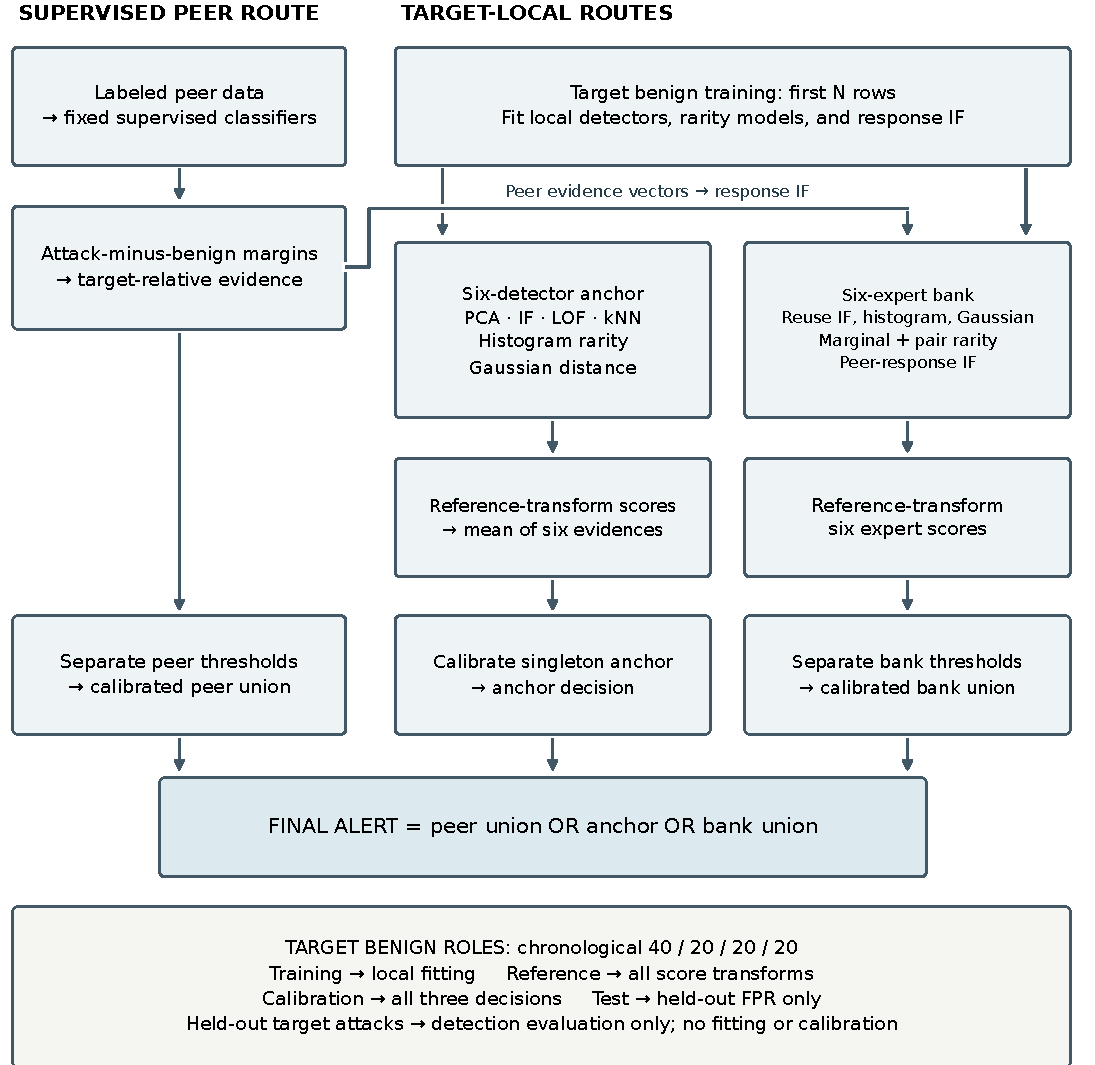
\includegraphics[width=\textwidth]{figures/architecture.pdf}
\caption{PACE's information flow and final decision. Target benign training, reference, calibration, and test roles are distinct. The benchmark standardizes features using pooled complete benign training roles before restricting local fitting to $N$ rows. Target attack labels enter evaluation only. IF: isolation forest; LOF: local outlier factor; $k$NN: nearest-neighbor distance.}
\label{fig:architecture}
\end{figure}

\subsection{Target-relative evidence}
For an expert score $s$, let $r_1,\ldots,r_n$ be that expert's scores on the target reference role, $r_{\max}=\max_i r_i$, and $d_R=\max\{r_{\max}-\operatorname{median}_i r_i,10^{-6}\}$. The implemented transformation is
\begin{equation}
 E_R(s)=\begin{cases}
 -\log\!\left(\dfrac{1+\sum_{i=1}^n\mathbf{1}\{r_i\geq s\}}{n+1}\right),&s\leq r_{\max},\\[6pt]
 \log(n+1)+\log\!\left(1+\dfrac{s-r_{\max}}{d_R}\right),&s>r_{\max}.
 \end{cases}
 \label{eq:evidence}
\end{equation}
Ties are included in the upper-tail count. Values beyond the largest reference score receive an extrapolated value, rather than a saturated empirical rank. This extrapolation is a score convention, not an estimated tail probability with a distribution-free validity guarantee. For peer $k$, the evidence is $e_k(x)=E_{R,k}(m_k(x))$.

\subsection{Blocks and thresholds}
Let $M=|C|$ and let $b=250$ be the configured block-size parameter. The code constructs $J=\max\{1,\lfloor M/b\rfloor\}$ consecutive blocks using a balanced array partition: their lengths differ by at most one, and earlier blocks receive any surplus rows. They are not necessarily blocks of exactly 250 observations. For example, 350 calibration observations form one block of length 350. Write $n_j=|C_j|$ and let $z_{j,(1)}\leq\cdots\leq z_{j,(n_j)}$ be ordered evidence in block $j$. For allocation $w\in(0,1)$,
\begin{equation}
 \tau_z(w)=\max_{1\leq j\leq J}
 z_{j,(1+\lceil(1-w)(n_j-1)\rceil)}.
 \label{eq:threshold}
\end{equation}
This is NumPy's higher empirical quantile followed by a maximum over blocks. Every decision uses a strict comparison $z(x)>\tau_z(w)$; equality does not alert. For a fixed threshold obtained this way, the observed exceedance fraction within each calibration block is at most $w$. This statement concerns the observations used to choose the threshold and does not extend to future data without additional assumptions.

\subsection{Separately calibrated experts and union scaling}
For a collection of $L$ experts with allocation $B$, the default initial shares are $w_\ell=B/L$. Given multiplier $\lambda$, the union is
\begin{equation}
 U_{B,\lambda}(x)=\mathbf{1}\!\left\{\exists\ell:
 z_\ell(x)>\tau_{z_\ell}(\lambda w_\ell)\right\}.
 \label{eq:union}
\end{equation}
The calibrator measures this union on every calibration block. Starting at $\lambda=1$, it doubles an upper search point until that point violates the block-rate criterion or reaches the allowed cap, returns immediately if the cap is feasible; otherwise it performs 20 bisections to retain a feasible lower point. The configured cap is 64. If the largest share times 64 is at least one, the implementation replaces the multiplier ceiling by $0.999/\max_\ell w_\ell$. If the initial union already violates $B$, the routine returns its initial thresholds; it does not claim to repair arbitrary supplied shares. PACE's equal-share initial unions satisfy the calibration criterion by the fixed-threshold count bound and the union bound.

The retained multiplier is a numerical search result on a stepwise calibration function. It should not be interpreted as a unique population optimum. The peer branch applies this routine to the $K$ separate margin-evidence experts with allocation $B_P$. Separate thresholds avoid collapsing all peer evidence into one maximum before calibration. The common multiplier nevertheless couples the thresholds through the observed union, so an unstable peer can still affect their joint calibration.

\subsection{Anchor and complementary local bank}
The anchor averages the reference-transformed scores of six local detectors: PCA reconstruction error, isolation forest, local outlier factor, mean nearest-neighbor distance, histogram rarity, and regularized Gaussian distance. Evidence is computed separately for each detector before averaging. The anchor is not transformed a second time. PCA retains 95\% of explained variance and uses mean squared reconstruction error. Isolation forest~\cite{liu2008isolation} uses 100 trees, local outlier factor~\cite{breunig2000lof} uses 20 neighbors, and the distance score averages 10 neighbor distances from the fitted neighbor structure. Histogram scores sum negative log smoothed bin frequencies across features, with 20 equal-width training bins and additive-one smoothing. Values outside a feature's training range use its minimum fitted bin probability. The Gaussian score is a squared Mahalanobis distance using a pseudoinverse of the sample covariance plus $0.001I$.

The local bank contains six experts. Three reuse the anchor members' isolation-forest, histogram, and Gaussian evidence. Two score feature rarity, and one scores the joint response of the peers. These feature experts reuse fitted detector outputs; they are not three additional independently fitted copies.

The first rarity expert sums two-sided empirical tail evidence. For feature $q$, let $a_q(v)$ count training values at most $v$ and $c_q(v)$ count training values strictly below $v$. Its raw score is
\begin{equation}
 s_{\mathrm{tail}}(x)=\sum_{q=1}^{d}\max\left\{
 -\log\frac{a_q(x_q)+1}{N+1},
 -\log\frac{N-c_q(x_q)+1}{N+1}\right\}.
 \label{eq:tail}
\end{equation}
This ECOD-inspired two-tail rarity score is labeled ECOD-sum in the implementation. It differs from original ECOD~\cite{ecod2022}, which maximizes three aggregate scores formed from left, right, and skewness-selected tails. Here the featurewise larger negative-log tail is selected before summation; the equation specifies the implemented variant.

For pair co-occurrence, 150 ordered feature-index pairs are drawn with replacement. Self-pairs are discarded when more than one feature is available; duplicate pairs can remain, so 150 is a draw count rather than a guaranteed count of distinct retained pairs. Each feature is coded using its unique internal training quantiles at levels $1/8,\ldots,7/8$, with left insertion at ties. Although these cut points give at most eight active codes, the implementation allocates a table of width $8+1=9$ in each dimension. If $h_{uv}(x)$ is the training count in the coded cell for retained pair $(u,v)$, the score is
\begin{equation}
 s_{\mathrm{pair}}(x)=\frac{1}{|\mathcal P|}\sum_{(u,v)\in\mathcal P}
 -\log\frac{h_{uv}(x)+0.5}{N+0.5\times9^2}.
 \label{eq:pair}
\end{equation}
The reference transformation in Eq.~\eqref{eq:evidence} is applied to both rarity scores.

The response expert fits a 100-tree isolation forest to vectors $\rho(x)=(e_1(x),\ldots,e_K(x))$ for $x\in T_N$. It uses the negative forest score as its anomaly score and then applies Eq.~\eqref{eq:evidence} relative to its scores on $R$. Thus it models how the collection of foreign classifiers responds to target benign data. It neither trains a gating network nor changes the supervised peer models.

\subsection{Resolution rule and final decision}
With anchor share $a=0.5$, the anchor allocation is
\begin{equation}
 B_A=\begin{cases}aB_L,&aB_L\geq1/b,\\B_L,&aB_L<1/b,\end{cases}
 \qquad B_B=(1-a)B_L.
 \label{eq:allocation}
\end{equation}
The anchor is itself calibrated by the union-scaling routine as a singleton expert with allocation $B_A$. The bank is separately calibrated as a six-expert union with allocation $B_B$. In particular, the anchor threshold is not merely the unscaled quantile $\tau_A(B_A)$. Let the resulting decisions be $U_P$, $U_A$, and $U_B$. The final rule is
\begin{equation}
 D(x)=U_P(x)\lor U_A(x)\lor U_B(x).
 \label{eq:final}
\end{equation}
There is no final calibration pass over this three-way union.

At $\alpha=0.01$ and $r=a=0.5$, these allocations are $B_P=0.005$, $B_A=0.005$, and $B_B=0.0025$. Their sum is 0.0125, rather than 0.01. At $\alpha=0.05$, they are 0.025, 0.0125, and 0.0125, whose sum is 0.05. Overlap and integer count resolution can make the observed calibration union smaller than the allocation sum, but do not justify presenting Eq.~\eqref{eq:allocation} as a strict partition of $\alpha$. The rule checks $1/b$, whereas the first possible nonzero exceedance for an individual higher quantile depends on its actual block length through $1/(n_j-1)$. The resolution rule is therefore an implemented heuristic, not an exact test of every block's quantile resolution.

The protected anchor preserves a separate local decision path but does not prove non-inferiority to the primary comparator. That comparator averages seven detector evidences, including an autoencoder omitted from the six-member anchor, and uses a different threshold procedure. Target-level regressions must be assessed empirically.

\begin{table}[tbp]
\centering
\begin{minipage}{0.96\textwidth}
\hrule\smallskip
\refstepcounter{algorithm}\textbf{Algorithm \thealgorithm. PACE preparation and inference}\label{alg:pace}
\smallskip\hrule\smallskip
\small
\textbf{Input:} fixed peer classifiers; target benign roles $T_N,R,C$; nominal $\alpha$; $r=a=0.5$; block parameter $b=250$.
\begin{enumerate}
\setlength{\itemsep}{2pt}\setlength{\parskip}{0pt}
\item Evaluate each peer's attack-minus-benign margins on $T_N,R,C$; construct reference transforms $E_{R,k}$ by Eq.~\eqref{eq:evidence}, including ties and beyond-reference extrapolation.
\item Fit the local detectors and rarity models on $T_N$, and the response IF on $(e_1,\ldots,e_K)(T_N)$. Transform each local score against its scores on $R$. Form the six-evidence mean anchor and six-expert bank.
\item Partition $C$ into $\max(1,\lfloor |C|/b\rfloor)$ balanced consecutive blocks. For each expert, use the maximum block higher quantile in Eq.~\eqref{eq:threshold}.
\item Set $B_P=(1-r)\alpha$ and $B_L=r\alpha$. Compute $B_A,B_B$ with the resolution rule in Eq.~\eqref{eq:allocation}.
\item Apply \textsc{CalibrateUnion} to the $K$ peers with $B_P$, the singleton anchor with $B_A$, and the six bank experts with $B_B$. Store all reference transforms and thresholds.
\item For a query $x$, compute the same frozen evidences. Alert if any peer exceeds its threshold, the anchor exceeds its threshold, or any bank expert exceeds its threshold. All comparisons are strict $>$; no final recalibration is applied.
\end{enumerate}
\textbf{CalibrateUnion}$(Z,B)$: initialize equal shares $w_\ell=B/L$ and thresholds at $\lambda=1$. Use cap $c=64$, replaced by $0.999/\max_\ell w_\ell$ if $64\max_\ell w_\ell\geq1$. Return the initial thresholds if their worst block union rate exceeds $B$. Otherwise test $\min(2,c)$ and double up to $c$ while feasible; return immediately if $c$ is feasible. Once an infeasible upper point is found, perform 20 bisections, retaining the feasible lower point. Return its thresholds.
\smallskip\hrule
\end{minipage}
\end{table}

\subsection{Training and computation}
Each peer classifier has two ReLU hidden layers of widths 64 and 16 and two output logits. Training uses class-balanced cross-entropy, Adam updates, eight epochs, batch size 256, and learning rate 0.001. Target-local fitting uses the first $N$ retained training rows. The feature-space isolation-forest and neighbor-based fitting sample is limited to 8000 rows; other local components have their own full-$N$ fitting operations. Fitted score references and thresholds are fixed at inference: the evaluated rule has no online update.

The benchmark's shared local ensemble also trains and scores an autoencoder for the mean-ensemble comparator, even though its score is excluded from PACE's anchor. It would therefore be inaccurate to describe the executed campaign as requiring no local neural training. The detection architecture requires $K$ peer forward evaluations plus local score computations; the response forest adds a model in $K$ dimensions. A peer MLP contains $64d+1138$ weights and biases for $d$ input features. This algebraic parameter count is not a measurement of serialization size, communication traffic, latency, energy use, or deployment memory. None of those operational quantities is established by the reported detection results.




\section{Experimental methodology}
\label{sec:experiment}
\subsection{Evaluation units and eligibility}
The evaluation contains six corpora organized into seven study strata: IoT-23~\cite{garcia2020iot23} (11 targets), TON\_IoT~\cite{moustafa2021ton} (9), Gotham~\cite{belarbi2025gothamdata} (7), CTU-13~\cite{garcia2014ctu} (12), N-BaIoT~\cite{nbaiot2018} (9), and UNSW IoT attack flows~\cite{hamza2019mud} G1 and G2 (5 each). These 58 units are the eligible benchmark targets, not a random sample of deployments. Each stratum uses its own compatible feature schema. Peer transfer occurs within the prepared pool for that stratum, rather than across corpora.

Reported-target membership is predefined by corpus-specific client manifests; eligibility is then checked within those manifests. A target must have at least one eligible attack type, at least 350 calibration observations, and at least four eligible peers. The configured minimum number of retained rows for an attack type is 600 by default, reduced to 400 for IoT-23, TON\_IoT, and CTU-13, and to 30 for the two UNSW strata. Eligibility therefore depends partly on the availability of evaluation attacks even though attack labels do not enter the target detector's fitting or calibration. This distinction matters when interpreting benign-only deployment claims.

The census records 769--80,000 benign training-role rows per target. Peer counts range from four in each UNSW group to eleven in CTU-13. Gotham's seven reported targets each have seven peers, indicating that reported-target and peer-pool membership must not be assumed identical. Corpus-specific preprocessing and retained sampling precede the experimental role split. Chronological ordering of retained observations is not equivalent to evaluation of an untouched continuous capture stream.

\begin{table}[tbp]
\centering
\small
\caption{Prepared target units and feature dimensions. Counts describe eligible reported targets; peer pools can be larger. Features and sampling are adapter-specific.}
\label{tab:corpora}
\begin{tabular}{llrr}
\toprule
Stratum & Evaluation unit & Targets & Features \\
\midrule
IoT-23 & Capture/scenario & 11 & 36 \\
TON\_IoT & Destination host & 9 & 29 \\
Gotham & Device capture & 7 & 37 \\
CTU-13 & Botnet scenario & 12 & 38 \\
N-BaIoT & Device directory & 9 & 115 \\
UNSW G1 & Device & 5 & 15 \\
UNSW G2 & Device & 5 & 13 \\
\bottomrule
\end{tabular}
\end{table}


Table~\ref{tab:corpora} distinguishes the evaluation units and input dimensions. TON\_IoT's selected destinations include routers, servers, and conventional hosts, so the collection should not be read as 58 consumer IoT devices. Each adapter applies a signed logarithmic feature transformation before pooled standardization. Sampling and eligibility operate on retained rows. IoT-23 caps each raw detail bucket at 200,000 benign or 60,000 malicious rows; TON\_IoT caps each host at 150,000 benign rows and each host--attack group at 60,000. IoT-23 additionally thins detail groups larger than 20,000 rows to 2\% within million-row chunks, only for files larger than 1.5 billion bytes. TON\_IoT thins host--label groups larger than 20,000 rows to 3\% within two-million-row chunks, using an intermediate 60,000-row reservoir. Both thinning counts are rounded down. CTU-13 retains at most 200,000 normal and 60,000 attack rows per scenario and discards Background traffic. Gotham retains at most 200,000 benign rows and 40,000 per attack type. N-BaIoT applies stable exact-row deduplication within files, and its source order substitutes for timestamps. The UNSW inputs use annotated minute-level flow counters and have no adapter reservoir cap.

Gotham's features require particular caution. Five features summarize all packets within each complete second, before label filtering and reservoir sampling. A retained benign row can therefore contain aggregate information about attack or unlabeled packets in that second, and later packets contribute to earlier rows' features. Role boundaries that divide a second do not separate the raw observations contributing to these aggregates. This dependency does not establish that attack labels entered model fitting, but it prevents interpreting the benchmark as immediate causal packet-stream detection.

\subsection{Role separation and fitting budgets}
The benign observations of each prepared client are ordered by timestamp or recorded source order, using a stable ordering. Split boundaries are the floors of the cumulative fractions 0.4, 0.6, and 0.8, producing training, reference, calibration, and test roles. The first $N$ training-role observations fit the local detectors. Insufficient rows cause the corresponding budget to be ineligible; observations are not borrowed from later roles to meet it.

For each eligible attack type, the ordered retained observations are divided at the midpoint. Up to the first 10,000 observations of the first half supply peer-development examples; up to the first 10,000 observations of the second half supply evaluation examples. A target's supervised model is omitted when that client becomes the monitored target. Other clients' development attacks remain available for peer training, including attack types that may also appear at the target. The experiment thus tests transfer to a target without attack labels, rather than a general guarantee of detection of attack families absent from all peer training. These chronological splits are applied separately within clients and labels; they do not impose a common wall-clock cutoff across the network.

The pooled standardizer is fitted before budget-specific local fitting, using complete benign training roles of the loaded clients. Reference and calibration roles remain separate from benign test rows in the decision pipeline. Nevertheless, this preprocessing means that the total target data available to the experiment exceeds $N$, as explained in Section~\ref{sec:problem}. Peer classifiers also use this common scaling, so target-derived benign statistics influence their input representation. No claim of fitting the entire system from 100 or 400 total target observations is made.

Four analyses avoid mixing changes in budget with changes in eligible targets. The universal primary analysis compares $N=100$ and $400$ on all 58 targets. Universal robustness adds $N=750$ on those same targets. Broad scaling compares $N=100$, $400$, and $2000$ within the 47-target cohort supporting 2000 rows. The high-resource analysis compares $N=100$, $400$, $2000$, and $20,000$ within the 15-target cohort supporting the largest budget. Budget effects are paired within their specified cohort.

\subsection{Configuration and comparison rules}
Both $\alpha=0.01$ and $0.05$ are evaluated. The reserve fraction is 0.5, the block-size parameter 250, the multiplier cap 64, and the bisection count 20. The learning seeds are 6, 7, and 8. Component seeds are derived by target identity and component domain; these runs vary learning randomness while keeping data roles fixed. The configuration's single default alpha is not the scope of the campaign: the protocol matrix explicitly includes both levels.

The primary comparator is PACE with a mean-ensemble local branch. Both methods use the same supervised peer architecture, target-relative peer evidence, peer calibration, target roles, learning-seed schedule, and evaluation cohort. The comparator thresholds the average evidence of seven local detectors at the full local allocation. The seventh detector is an autoencoder with hidden widths 20 and 10, a symmetric decoder, 30 training epochs, batch size 256, and learning rate 0.001. This comparator differs from the six-member anchor in both composition and calibration, so the primary comparison is an assessment of the complete local-branch replacement.

Two recorded baselines also retain this seven-detector local branch. The max-fusion baseline transforms peer attack probabilities relative to target reference probabilities, takes their maximum, and calibrates that fused value once. Its beyond-reference transformation differs from the margin transformation in Eq.~\eqref{eq:evidence}: it adds the logarithm of the probability-to-reference-maximum ratio to $\log(n+1)$. The Bonferroni baseline uses equally shared margin-evidence peer thresholds with multiplier fixed to one. These baselines should not be described as peer-only detectors.

Separate peer-mean and peer-maximum ablation arms fuse PACE's margin evidence while retaining the PACE local bank. These arms distinguish the effect of fused peer calibration from the probability-based recorded max-fusion baseline. The no-local-channel arm allocates the entire nominal parameter to the peer union, whereas the reported peer branch inside PACE receives only its reserved peer share. The local-only arm uses the seven-detector mean at the entire nominal parameter. Neither standalone arm is identical to a branch extracted from the final combined rule.

Additional arms remove the feature, rarity, or response family; remove the anchor; combine anchor and bank into a single weighted union; fit the response expert on margins; or reduce the local reserve to 0.25. Every arm uses the same relevant data roles and seed schedule. These are internal architectural comparisons. The campaign does not provide implementations of every contemporary federated, transfer, or calibrated intrusion detector, so literature positioning is not an empirical superiority comparison with those methods.

\subsection{Metrics and aggregation}
For target $t$, attack type $h$, and seed $s$, detection is the fraction of held-out attack observations that alert. The target detection rate averages these fractions equally across its attack types and then across the three seeds. The pooled detection rate averages targets equally. Large captures therefore do not dominate through their row counts, although strata with more targets have greater pooled weight. False-alert rate is the fraction of benign test observations that alert, averaged over seeds within target and then over targets for its pooled mean.

The primary paired difference subtracts the comparator's target detection from PACE's. Intervals use 10,000 bootstrap replicates with seed 314159 and confidence level 0.95. Targets are sampled with replacement within corpus groups identified by the dataset enum, preserving each group's size, and their contributions are weighted by target count. The interval endpoints are linear empirical quantiles of the bootstrap means. The two UNSW study strata belong to one corpus group for this resampling. Seeds and attack observations are not resampled as independent targets.

This procedure conditions on the observed corpora and the seed-averaged target effects. It does not account fully for shared peer models, common captures, cohort selection, or dependence between target units. Intervals are descriptive evidence about this benchmark; they are not uncertainty bounds for arbitrary new IoT populations. Multiple ablations and subgroup analyses are exploratory, without a claim of simultaneous family-wise coverage.

Sweep-adjusted primary comparisons use multipliers $\{0.55,0.75,1,1.4\}$ at $\alpha=0.01$ and $\{0.4,0.75,1,1.4\}$ at $\alpha=0.05$, scaling both branch allocation parameters. PACE's complete rule, including its resolution condition, is evaluated at each stored point. Primary reporting interpolates within the realized-rate sweep and clamps outside its endpoints, separately for each seed. This procedure approximates a comparator operating point; it does not guarantee exact matching. The false-alert distribution reports quantiles over target seed means, while acceptance additionally examines exceedance among target--seed cells. These denominators are distinct.

\subsection{Internal protocol checks and reproducibility}
The primary engineering acceptance rule permits no target loss exceeding 0.05 and permits at most 3\% of targets to lose more than 0.01. It also requires positive lower bounds for nominal and sweep-adjusted pooled gains; limits mean false-alert increases to 0.004 or 0.002 at the two alpha levels; limits the increase in target--seed exceedance above $2\alpha$ to 0.03; and checks excluded-TON\_IoT, learning-seed, and leave-one-stratum-out summaries. These conditions describe the repository's decision rule. They do not constitute a formal non-inferiority hypothesis test, a registered clinical-style margin analysis, or external validation.

The outcome-independent power table is a planning calculation over assumed paired standard deviations and a meaningful effect of 0.02, using level 0.05 and power 0.8. It is not an observed-power validation of the results. At 58 targets, for example, assumed standard deviations of 0.05 and 0.10 produce minimum detectable effects of 0.018393 and 0.036787. The conclusions rely on the actual paired outcomes and their limitations rather than on selecting a favorable planning assumption.

All numerical summaries reported here are taken from the existing campaign tables. No models were retrained and no scientific campaign was rerun during manuscript preparation. Held-out learning seeds assess the fixed design within the reported cohort. Provenance checks establish artifact identity and consistency; they do not extend the evaluation to other target populations.





\section{Experimental results}
\label{sec:results}
\subsection{Does the local bank improve the primary comparator?}
Table~\ref{tab:primary} reports the universal primary cohort of 58 targets. The comparator retains the same peer branch but uses a single mean of seven local detector evidences. At nominal $\alpha=0.01$, replacing that local branch with PACE raises mean detection from 0.807318 to 0.833405 at 100 local fitting rows and from 0.810681 to 0.838987 at 400 rows. The paired gains are 0.026086 and 0.028306. At $\alpha=0.05$, the corresponding gains are 0.023418 and 0.023219. All four corpus-stratified bootstrap intervals exclude zero.

These are absolute differences in target-macro detection rate, not relative percentage improvements or estimates of packet-weighted operational detection. The intervals describe resampling of the observed target differences within the available corpus strata. They do not incorporate uncertainty from choosing new corpora or from cohort selection.

\begin{table}[tb]
\centering\small
\caption{Universal primary comparison with the mean-ensemble local branch, 58 targets. Intervals are 95\% corpus-stratified paired bootstrap intervals. Detection rates are averaged over attack types, learning seeds, and targets.}
\label{tab:primary}
\begin{tabular}{rrrrl}
\toprule
$\alpha$ & $N$ & PACE & Comparator & Gain [95\% interval]\\
\midrule
0.01 & 100 & 0.833405 & 0.807318 & 0.026086 [0.011323, 0.043346]\\
0.01 & 400 & 0.838987 & 0.810681 & 0.028306 [0.012339, 0.047375]\\
0.05 & 100 & 0.894767 & 0.871348 & 0.023418 [0.005777, 0.043968]\\
0.05 & 400 & 0.896837 & 0.873619 & 0.023219 [0.003116, 0.045968]\\
\bottomrule
\end{tabular}

\end{table}

The nominal comparison is not a comparison at equal realized false-alert rates. At $\alpha=0.01$, PACE increases the mean false-alert rate by 0.003476 at 100 rows and 0.001588 at 400 rows. At $\alpha=0.05$, it reduces it by 0.001984 and 0.010070. Thus the detection gains at the smaller nominal operating parameter partly accompany increased benign alerts. At the larger parameter, the mean detection and mean false-alert differences both favor PACE, although averages alone do not establish dominance for individual targets.

\subsection{How much remains after operating-point adjustment?}
The stored budget sweep yields primary comparator-adjusted gains of 0.024659, 0.025735, 0.022176, and 0.020718 for the four settings in Table~\ref{tab:primary}. The four intervals, in the same order, are $[0.009682,0.042034]$, $[0.009690,0.044983]$, $[0.005135,0.042086]$, and $[0.002056,0.042482]$. These estimates remain positive, but their interpretation requires the actual interpolation procedure.

For each target and learning seed, the reporting code sorts PACE's four sweep points by realized benign false-alert rate and linearly interpolates detection at the comparator's rate. When that rate falls outside the observed sweep, the calculation uses the nearest endpoint. It then averages the resulting differences over seeds and targets. Consequently, these figures are clamped sweep-adjusted comparisons, not evidence that every detector was evaluated at precisely the same false-alert rate. The primary calculation also differs from a separate max-fusion reporting routine that constructs a monotone envelope and rejects uncovered operating points. Claims about primary matched comparisons must use the former definition. The narrow four-point sweep and endpoint handling limit how much this analysis can resolve operating-point confounding. Of 174 target--seed cells per setting, the comparator rate falls below or above the PACE sweep in 47/28 cells at $\alpha=0.01$, $N=100$, and 49/20 cells at $N=400$. At $\alpha=0.05$, these counts are 12/24 and 9/19. Thus 75, 69, 36, and 28 comparisons respectively use endpoints outside the covered range. These counts are derived from the stored campaign sweeps; they make explicit how often the reported adjustment cannot actually match the comparator rate.

\subsection{Are false alerts compatible with the nominal parameter?}
Table~\ref{tab:fpr} gives the distribution of target false-alert rates after averaging over learning seeds. At $\alpha=0.01$, PACE's mean is 0.033992 at 100 rows and 0.032369 at 400 rows, while the medians are 0.006485 and 0.006419. The large difference between means and medians indicates substantial heterogeneity. The worst target averages are 0.669005 and 0.670842. About 26\% of targets exceed twice the nominal parameter in both settings. A nominal value of 0.01 therefore cannot be interpreted as a one-percent test-time false-alert bound.

\begin{table}[tb]
\centering\small
\caption{Distribution of PACE's target-level realized false-alert rates, averaged over three learning seeds. Exceedance columns are proportions of targets, not proportions of individual benign rows or target--seed cells.}
\label{tab:fpr}
\begin{tabular}{rrrrrrrr}
\toprule
$\alpha$ & $N$ & Mean & Median & 90th pct. & Worst & $>\alpha$ & $>2\alpha$\\
\midrule
0.01 & 100 & .033992 & .006485 & .062058 & .669005 & .413793 & .258621\\
0.01 & 400 & .032369 & .006419 & .067903 & .670842 & .396552 & .258621\\
0.05 & 100 & .055453 & .019118 & .162115 & .671844 & .224138 & .137931\\
0.05 & 400 & .054337 & .018427 & .159692 & .671844 & .241379 & .137931\\
\bottomrule
\end{tabular}

\end{table}

The comparator has the same qualitative failure: at $\alpha=0.01$, its mean rates are 0.030516 and 0.030781, and its worst-target rates are 0.670174 and 0.670842. This shared failure does not excuse PACE's additional alerts. It shows that calibration on earlier benign data is insufficient to deliver the nominal rate on the later benign role in this benchmark. The results alone cannot assign the discrepancy to a unique cause, such as temporal shift, sample selection, or score extrapolation. Moreover, the resolution rule's allocation sum already exceeds 0.01 before considering any test-distribution change.

At $\alpha=0.05$, PACE's means are 0.055453 and 0.054337; the corresponding 90th percentiles are 0.162115 and 0.159692. The worst value remains 0.671844. Even where the pooled average approaches the nominal parameter, the upper tail is unsuitable evidence for uniform operational control. A row-level false-alert rate is also not an incident-level alert burden: aggregation, duplicate suppression, analyst capacity, and the benign-to-attack prevalence of a deployed stream were not measured.

Figure~\ref{fig:false-alerts} shows the complete cumulative distributions, including the long upper tails that are obscured by pooled means.
\begin{figure}[p]
\centering
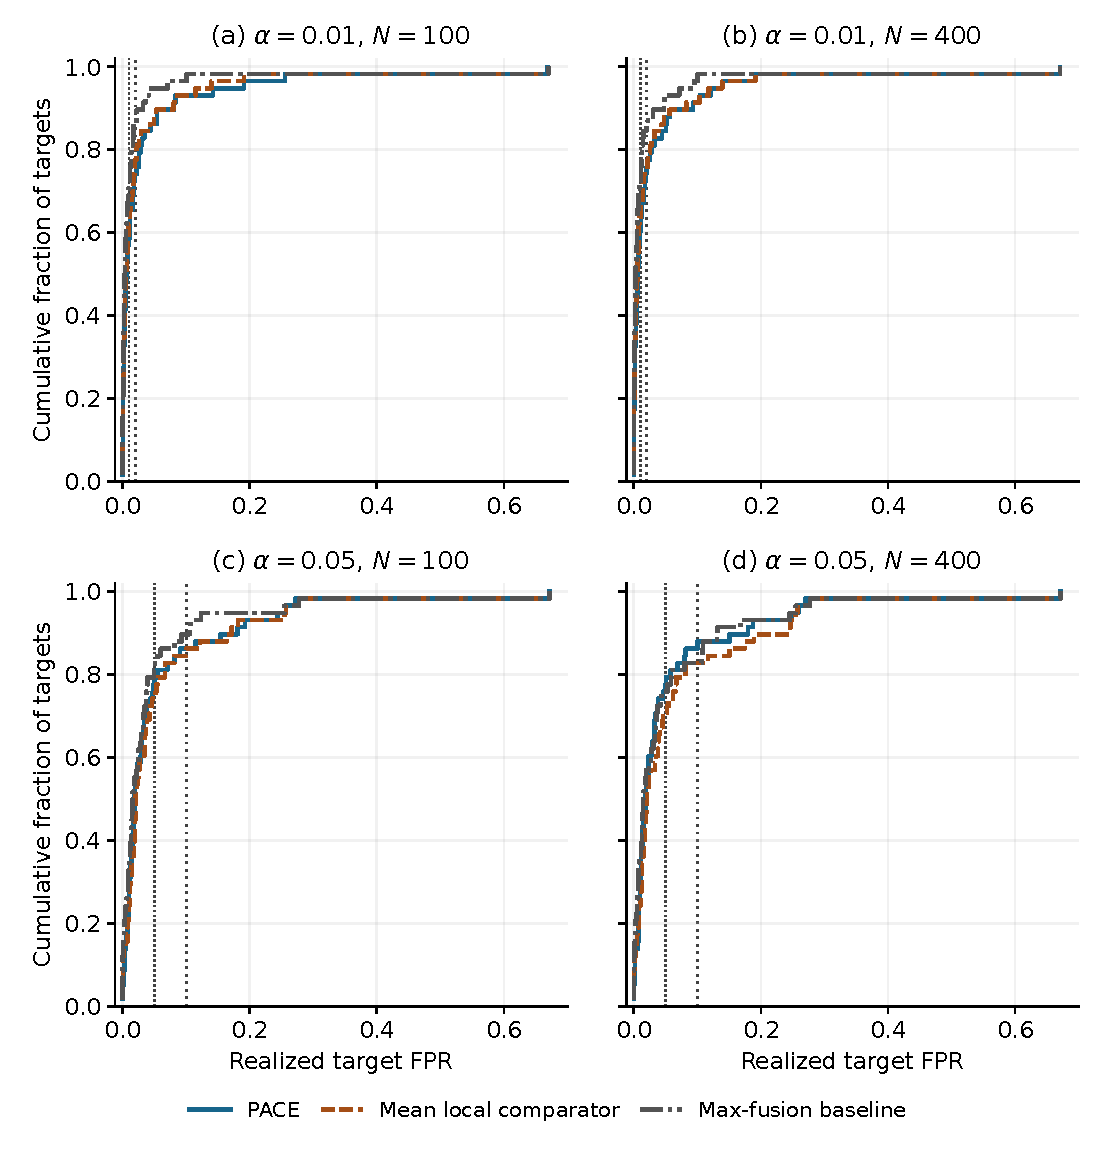
\includegraphics[width=\textwidth]{figures/false-alert-distribution.pdf}
\caption{Empirical cumulative distributions of benign test false-alert rates for 58 targets, after averaging each target over three learning seeds. Dashed vertical guides mark $\alpha$ and $2\alpha$; they are nominal reference values, not demonstrated bounds. The recorded max-fusion baseline includes the mean-ensemble local branch. Curves reproduce the frozen figure unchanged; color distinguishes methods, while Table~\ref{tab:fpr} supplies numerical PACE distribution summaries independently of color.}
\label{fig:false-alerts}
\end{figure}
\subsection{Where are the gains concentrated?}
TON\_IoT has the largest stratum mean gains: 0.117448 and 0.126729 at $\alpha=0.01$, and 0.120780 and 0.104447 at $\alpha=0.05$, for 100 and 400 fitting rows respectively. Removing its nine targets reduces the pooled gains to 0.009306, 0.010228, 0.005536, and 0.008299. Their intervals are $[0.001808,0.019526]$, $[0.000995,0.024240]$, $[0.000090,0.014343]$, and $[0.000143,0.022250]$. The remaining gains are positive in these primary summaries but small, and two lower bounds lie very close to zero.

N-BaIoT is already near complete detection and changes by approximately $10^{-5}$ or less. Gotham gains range from 0.001950 to 0.005907. UNSW G2 improves by 0.009251 and 0.005548 at $\alpha=0.01$, but changes by $-0.001420$ and $-0.002037$ at $\alpha=0.05$. Several stratum intervals include zero. The median target gain is zero in many strata, so a positive mean should not be paraphrased as an improvement for most devices.

IoT-23's primary mean gains range from 0.017582 to 0.029670, but its target-level pattern is concentrated rather than uniform. At $\alpha=0.01$ and 400 rows, CTU-13's mean gain is 0.003156 with interval $[-0.007871,0.017066]$. Scenario 12 loses 0.032595, the only primary target loss exceeding 0.01. No primary target loses more than 0.05. The comparator's autoencoder and PACE's different anchor composition are possible contributors to this regression; the final ablation set does not isolate a causal attribution to the autoencoder alone.

Figure~\ref{fig:targets} displays the concentration of the gains and the negative tail without aggregating targets into stratum means.
\begin{figure}[p]
\centering
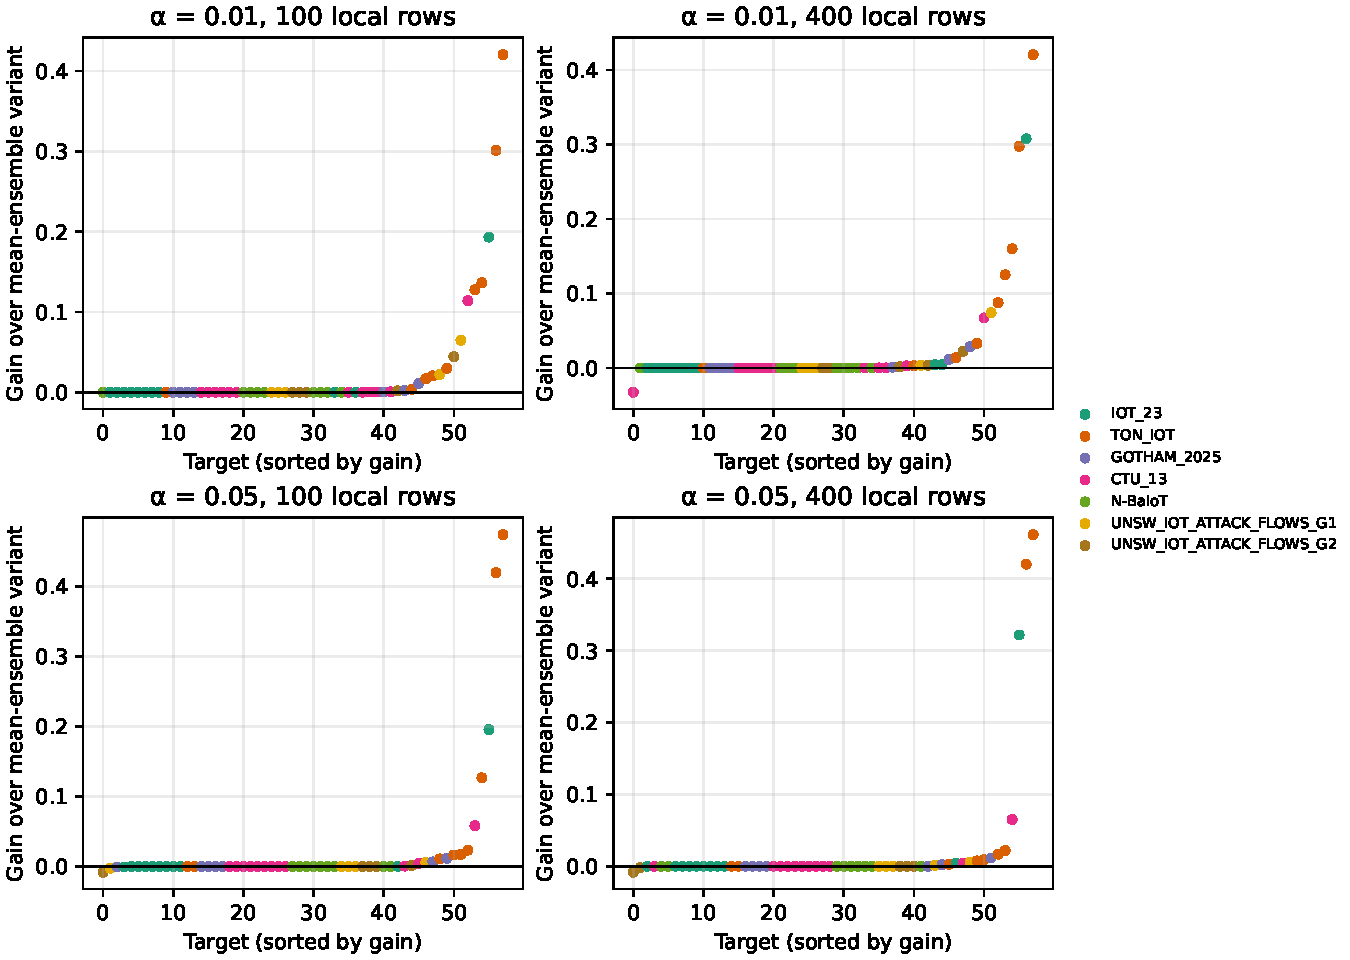
\includegraphics[width=\textwidth]{figures/target-gains.pdf}
\caption{Target-level detection differences, PACE minus the mean-ensemble local comparator. Each panel independently sorts its 58 seed-averaged target differences; a horizontal position is a rank, not a shared target identity across panels. Colors identify study strata. The overall concentration and negative differences remain visible in grayscale; stratum attribution requires the legend colors and is described numerically in the text. Axes report absolute detection-rate differences, not percentages.}
\label{fig:targets}
\end{figure}
\subsection{Which components supply complementary detections?}
Removing the rarity family costs 0.008626 and 0.011977 in pooled detection at $\alpha=0.01$, compared with 0.003413 and 0.002013 for removing feature experts, and 0.002008 and 0.002796 for removing the response expert. At $\alpha=0.05$, the rarity costs remain 0.006020 and 0.010403; feature costs are only 0.000127 and 0.000344. The response expert's costs are 0.003118 and 0.001269. These results support a modest complementary contribution, especially from rarity, rather than identifying response-space modeling as the main source of the improvement.

Ablation changes also recalibrate the remaining union. They are not additive decompositions of the gain and cannot be summed to assign causal importance. Replacing target-relative peer responses by raw margins changes pooled detection by only 0.001101--0.002879 across primary settings. Several corresponding intervals include zero. The evidence for the particular response representation is therefore weaker than the overall comparison with the mean-ensemble local branch.

The anchor has a tradeoff. Removing it reduces mean detection at $\alpha=0.01$, but the corresponding intervals include zero. At $\alpha=0.05$, the bank without the anchor detects more: its rates are 0.897598 and 0.898372, versus PACE's 0.894767 and 0.896837. Its false-alert rates are also higher, at 0.060458 and 0.064650. A single local union gives identical detection to PACE at $\alpha=0.01$ to the precision of the stored table; at $\alpha=0.05$ its differences are small and its false-alert rates higher. These outcomes do not establish that the tier structure is uniformly superior.

Within the final PACE rule, the attack-detection decomposition distinguishes alerts unique to the local branch from detections shared with peers. At $\alpha=0.01$ and 400 rows, local-exclusive detection is 0.147434 in TON\_IoT and 0.120957 in IoT-23, but only 0.000042 in N-BaIoT. These quantities are coverage fractions within the final rule, not gains over the mean-ensemble comparator and not the performance of a separately calibrated local-only detector.

\subsection{Does more local fitting data reliably help?}
On the same 58 targets, increasing the fitting budget from 100 to 400 rows changes PACE detection by 0.005582 at $\alpha=0.01$, with interval $[-0.003760,0.015387]$, and by 0.002070 at $\alpha=0.05$, with interval $[-0.004456,0.008690]$. Neither interval excludes zero. The local branch alone gains much more coverage, but much of that coverage overlaps detections already supplied by peers. The combined rule need not improve proportionally to the local branch.

At 750 rows, the universal cohort retains gains over the comparator of 0.024276 and 0.022614. However, at $\alpha=0.05$, the interval for the gain excluding TON\_IoT includes zero. The 2000-row analysis contains only the 47 targets with enough training-role observations. Its gains over the comparator are 0.019624 and 0.007358; both sweep-adjusted intervals include zero. At $\alpha=0.05$, the gain excluding TON\_IoT is negative, $-0.000370$, with interval $[-0.000712,-0.000074]$.

The 20,000-row cohort contains 15 targets. Its nominal gains are 0.005329 at $\alpha=0.01$ and $-0.001311$ at $\alpha=0.05$, with intervals including zero. Within this cohort, increasing the budget from 100 to 20,000 rows at $\alpha=0.05$ reduces PACE detection by 0.028296, with interval $[-0.032827,-0.023766]$. The results therefore do not support monotonic improvement with additional local fitting data. Comparisons across the 58-, 47-, and 15-target cohorts would confound fitting budget with target composition and are not used as estimates of budget effects.

Figure~\ref{fig:budgets} summarizes comparator gains within each fixed resource-eligible cohort.
\begin{figure}[tbp]
\centering
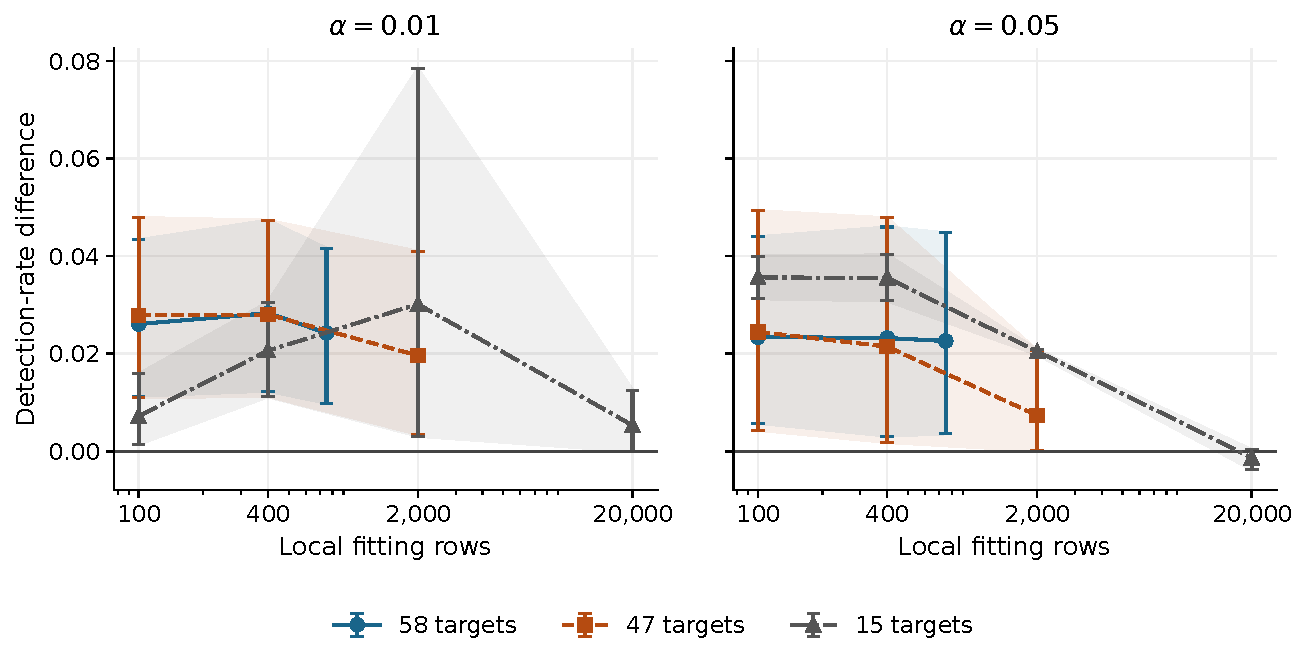
\includegraphics[width=\textwidth]{figures/budget-scaling.pdf}
\caption{Detection gain over the mean-ensemble local comparator as a function of local fitting rows on a logarithmic horizontal axis. The universal primary and robustness cohorts contain the same 58 targets; their curves overlap at shared budgets. Broad scaling uses 47 targets and the plotted ``extreme high-resource'' analysis uses 15. Shading gives 95\% corpus-stratified bootstrap intervals at evaluated budgets; connecting lines and bands are visual guides, not additional experiments. Compare budgets within a curve; differences between curves also reflect cohort composition. Color identifies cohorts; numerical findings in the text give the principal trends independently of color.}
\label{fig:budgets}
\end{figure}
\subsection{Seed stability and engineering acceptance}
Every learning seed has a positive primary pooled gain, ranging from 0.015977 to 0.039551 across settings. This consistency is narrower than generalization to new targets: all three seeds reuse the same data and splits. Excluding TON\_IoT, seed 6 has a gain of $-0.000195$ at $\alpha=0.05$ and 400 rows. Every primary leave-one-study-stratum-out pooled gain is positive, but this sensitivity check still operates on the same collection of corpora and targets.

The primary cells satisfy the repository's engineering acceptance criteria, which permit a limited fraction of harmed targets, bound changes in realized false alerts, and require positive aggregate summaries. This is not a formal statistical non-inferiority test or independent external validation. In particular, the observed scenario-12 regression remains a regression despite satisfying the aggregate acceptance rule. The larger-budget non-gating analyses contain failures of individual criteria and are reported as such, rather than being used to extend the primary verdict.




\section{Discussion}
\label{sec:discussion}
\subsection{Complementary local coverage}
The principal benefit of the heterogeneous local branch is complementary coverage. Under the final OR rule, locally detected attacks improve the combined decision only when the supervised peer union misses them. This explains why the gains depend on the availability of peer-missed attacks and why improved standalone local detection need not translate into proportional end-to-end gains. Local-exclusive coverage at $\alpha=0.01$ and $N=400$ reaches 14.74\% in TON\_IoT and 12.10\% in IoT-23, whereas it is nearly zero in N-BaIoT.

The rarity-family removals produce the largest detection losses among the tested expert-family ablations in all four primary configurations. This supports the usefulness of marginal and pairwise feature-rarity evidence alongside the shape- and neighborhood-based detectors. The smaller response-expert effects indicate that joint peer-response modeling supplies additional, but less extensive, coverage. Because each removal recalibrates the remaining union, the losses characterize complete ablated rules rather than an additive attribution to individual experts.

The protected anchor preserves an averaged local decision path alongside sparse expert alerts. Its value is an operating tradeoff: at $\alpha=0.05$, removing it raises both detection and false alerts. The primary comparison also changes the comparator's seven-member composition and thresholding, so the overall gain belongs to the complete local-branch replacement.

\subsection{Retaining peer evidence separately}
Peer-wise calibration gives each classifier its own target-relative threshold. Unlike a threshold on a fused maximum, a high threshold for one peer need not directly exclude another peer's smaller evidence. This addresses the peer-drowning mechanism while retaining dependence through the common union multiplier.

The peer-fusion ablations retain the PACE local bank and test this architectural choice separately from the primary local-branch comparison. At $\alpha=0.01$, PACE exceeds peer-mean fusion by 7.34 and 5.60 percentage points and peer-maximum fusion by 4.56 and 3.64 points at $N=100$ and $400$. At $\alpha=0.05$, the corresponding advantages are 5.25 and 4.47 points over the mean, and 3.05 and 3.16 over the maximum. All eight paired intervals exclude zero. The fused arms also have lower mean FPR: 0.023855--0.026093 at $\alpha=0.01$ and 0.043049--0.047157 at $\alpha=0.05$, compared with PACE's 0.032369--0.033992 and 0.054337--0.055453. These results support a detection advantage at the tested nominal parameters, accompanied by an alert-rate tradeoff.

The shared multiplier uses overlap between calibration alerts to relax thresholds while checking their union on every block. It does not require independent peer alerts. It also couples the retained thresholds, since changing one expert's calibration alerts can change the multiplier for all peers. The empirical evidence transformation and union search retain the calibration interpretation specified in Section~\ref{sec:method}.

\subsection{Variation across targets and fitting budgets}
TON\_IoT offers the largest observed gain and substantial local-exclusive coverage. IoT-23 also benefits on average, although its gains are concentrated in a subset of targets. N-BaIoT's near-complete peer coverage leaves little room for the local path to improve the final union. CTU-13 has small and uncertain stratum gains and includes the scenario-12 regression. These outcomes locate the empirical value of complementarity without attributing corpus differences to unmeasured traffic properties.

Increasing local fitting data changes the learned local evidence, but the final detector benefits only from changes outside existing peer coverage. On the fixed 58-target cohort, moving from 100 to 400 rows produces small, uncertain end-to-end changes; the 750-row comparison still favors PACE over the comparator. Benefits are weaker in the 47-target and 15-target resource-eligible cohorts, and the high-resource $\alpha=0.05$ budget change is negative. Consequently, neither larger budgets nor higher standalone local coverage imply monotonic improvement of the final OR rule.

\subsection{Practical interpretation}
At $\alpha=0.05$, PACE's primary detection gains accompany lower mean FPR at both budgets. Operational assessment must additionally consider the target distribution: at $\alpha=0.01$, medians below 0.01 coexist with means above 0.03 and worst-target rates near 0.67. The mean improvement is useful comparative evidence, while the upper tail shows why the nominal parameter cannot serve as a uniform operational guarantee.

Applying the detector requires trusted benign onboarding data for fitting, reference construction, and calibration, plus the preprocessing access in Table~\ref{tab:data-access}. References and thresholds remain fixed in the evaluated rule. Independent validation would need to establish when to update them, how to respond to excessive alerts, and how any recalibration changes detection.

Row alerts also require a policy for aggregation into actionable incidents. An anomalous record need not represent an actionable security event~\cite{sommer2010closed}, and precision depends on attack prevalence~\cite{saito2015precision}. The benchmark's separately sampled classes and target-macro rates do not measure incident precision or analyst workload. These operational questions remain distinct from the demonstrated detection contribution.

\section{Threats to validity and limitations}
\label{sec:limitations}
\paragraph{Evaluation population and dependence}
The 58 eligible targets are not a random deployment sample. Eligibility requires evaluation attacks, sufficient benign calibration data, and enough peers; larger-budget cohorts additionally select for abundant retained training data. Targets can share peer models, captures, collection conditions, and attack-generation procedures. The corpus-stratified bootstrap conditions on the observed corpus groups and does not fully model these dependencies. Three learning seeds assess a fixed design on the same cohort, which was also used during development; they do not sample new corpora. Subgroup and ablation intervals are exploratory, without simultaneous coverage. These boundaries follow established concerns about selection and laboratory evaluation in security machine learning~\cite{arp2024pitfalls}.

\paragraph{Information availability and preprocessing}
Dataset annotations identify the benign onboarding roles. Obtaining equally trustworthy observations in deployment remains an assumption, alongside labeled peer attacks and compatible feature schemas. Additional reference and calibration data and full-training-role pooled standardization make $N$ a local fitting budget rather than a total onboarding budget. Gotham's complete-second aggregates can include attack or unlabeled packets, allow later packets to influence earlier rows, and share raw contributors across role boundaries (Section~\ref{sec:experiment}). This dependency differs from direct use of attack labels in target fitting. Corpus-specific sampling, deduplication, and source ordering further limit chronological interpretation; separate client and label streams do not establish a network-wide prospective cutoff.

\paragraph{Calibration and distribution change}
Calibration controls empirical block rates, without establishing future FPR bounds. The low-alpha allocation exception, reference-tail extrapolation, and final OR without recalibration are part of the implemented rule. Target-level FPR heterogeneity remains substantial under this rule. No online drift detector, adaptive reference update, or recalibration policy was evaluated, and future traffic need not share the calibration distribution.

\paragraph{Comparison and attribution}
The primary comparator changes a complete local branch, including detector composition and calibration. Removal ablations also recalibrate the retained experts. They do not isolate every detector's causal contribution or establish optimality of the allocation. Contemporary external competitors, including MCDE, were not executed under the same protocol; the related-work comparison establishes methodological distinctions, not performance superiority. Attack families can occur in peer development data, so the target information restriction is not uniformly an unseen-attack-family test. Transfer is within compatible study strata, not across corpus schemas.

\paragraph{Security and operational deployment}
The study assumes trustworthy peers and does not test adversarial-peer behavior, poisoning, evasion, encrypted-feature availability under operational constraints, or attacks on the monitor. Model combination and centralized pooled preprocessing establish no privacy guarantee. End-to-end latency, throughput, memory, energy, communications, incident handling, and online deployment were not measured. The shared benchmark pipeline trains the comparator's autoencoder even though PACE excludes its output; algebraic model sizes cannot substitute for measurements of an eventual deployment implementation.

\section{Conclusion}
PACE combines separately calibrated supervised peer classifiers with a protected local anchor and a heterogeneous bank of anomaly experts for targets that provide benign observations but no attack labels. Across 58 benchmark targets, replacing a seven-detector mean local branch improves target-macro detection in all four primary configurations. The gains range from approximately 2.32 to 2.83 percentage points; at nominal $\alpha=0.05$, they accompany lower mean realized false-alert rates. This is the strongest evidence for the complete local-branch replacement. Rarity-family removal produces the largest detection loss among the tested expert-family ablations, and local-exclusive coverage identifies where local experts add detections beyond the peer union. Separately retained peer decisions also improve detection over mean or maximum peer fusion, with a higher mean false-alert rate.

The contribution is an empirically evaluated architecture for complementary peer and local detection under benign-only target fitting and calibration. Gains are concentrated in TON\_IoT, are smaller in several other strata, and do not consistently increase with larger local fitting budgets. The cohort also informed development, and heterogeneous realized false-alert rates limit operational interpretation. The results support the measured architectural tradeoffs; validation on untouched traffic is needed to establish their generality and acceptable false-alert behavior in deployment.

\section*{Data and code availability}
The evaluation uses the existing PACE implementation and frozen experimental outputs. A public code archive, immutable release identifier, dataset access links, and applicable redistribution conditions must be confirmed by the authors before submission. No public release is asserted in this draft.
\section*{Funding and competing interests}
Funding sources and competing-interest declarations require confirmation by the authors. No absence of funding or competing interests is inferred.
\section*{Authorship and acknowledgements}
Author names, affiliations, corresponding-author details, contribution statements, and acknowledgements remain to be supplied and approved by the authors.
\section*{Declaration of generative AI and AI-assisted technologies in the manuscript preparation process}
OpenAI Codex was used for repository inspection, literature assistance, manuscript drafting, and technical verification. This draft requires human scientific review and approval. The authors must confirm the extent of their review and responsibility for the final content before submission; this draft does not assert that such approval has already occurred.
\bibliographystyle{elsarticle-num}
\bibliography{references}
\end{document}


